\documentclass{jcgt}

\usepackage{amsmath}
\usepackage{listings}
\usepackage{xcolor}
\usepackage[normalem]{ulem}
\usepackage{siunitx}
\usepackage{csquotes}
\usepackage{url}
\usepackage{subcaption}
\usepackage{xcolor}
\usepackage{algorithm}
\usepackage{algorithmicx}
\usepackage{algpseudocode}
\usepackage{mathtools}
\usepackage{xfrac}
\usepackage{comment}
\usepackage{natbib}
\usepackage[font={small,it}]{caption}
\usepackage{tikz}
\usetikzlibrary{positioning}

\usepackage[export]{adjustbox}

\setciteauthor{Matthias Raab and Laurent Belcour and Frankie Liu and Jamie Portsmouth}
\setcitetitle{The Minimal Retroreflective Microfacet Model (MRM)}
%\setheadtitle{Abbreviated title, only if full title won't fit in page headers}

% Mark submissions with the date of submission using the following line:
\submitted{\today}

% Once an article is accepted accepted, switch to the following line and comment the preceding one. The editor will supply the argument values.
%\accepted{yyyy-mm-dd}{yyyy-mm-dd}{yyyy-mm-dd}{Editor Name}{volume}{issue}{1}{6}{yyyy}
\seturl{http://jcgt.org/published/vol/issue/num/}
\newcommand{\vecv}{\mathbf{v}}
\newcommand{\vecvv}{\mathbf{v'}}
\newcommand{\vecl}{\mathbf{l}}
\newcommand{\vecll}{\mathbf{l'}}
\newcommand{\vecn}{\mathbf{n}}
\newcommand{\vecm}{\mathbf{m}}
\newcommand{\vech}{\mathbf{h}}
\newcommand{\vechr}{\mathbf{h_r}}
\newcommand{\vecht}{\mathbf{h_t}}
\newcommand{\vecb}{\mathbf{b}}
\newcommand{\vecbr}{\mathbf{b_r}}
\newcommand{\vecbt}{\mathbf{b_t}}
\newcommand{\vecx}{\mathbf{x}}
\newcommand{\vecxx}{\mathbf{x'}}
\newcommand{\vecy}{\mathbf{y}}
\newcommand{\vecyy}{\mathbf{y'}}
\newcommand{\etav}{\eta_{\mathbf{v}}}
\newcommand{\etal}{\eta_{\mathbf{l}}}
\newcommand{\etax}{\eta_{\mathbf{x}}}
\newcommand{\etay}{\eta_{\mathbf{y}}}
\newcommand{\vdot}[2]{\left\langle #1, #2 \right\rangle}
%\newcommand{\vdot}[2]{#1\cdot#2}
\newcommand{\avdot}[2]{\lvert\vdot{#1}{#2}\rvert}

\newcommand{\laurent}[1]{{\color{blue}\textbf{[Laurent:} #1\textbf{]}}}

\includecomment{introduction}
\includecomment{existing-models}
\includecomment{eon}
\includecomment{eon-sampling}
\includecomment{conclusion}

\urlstyle{same}

\captionsetup[table]{skip=10pt}

\lstdefinestyle{snippet}{
  float=tp,
  floatplacement=tbp,
  abovecaptionskip=5pt
}

\lstdefinelanguage{GLSL}%
{%
	morekeywords={%
	% HLSL constants
		false,FALSE,NULL,true,TRUE,%
	% GLSL predefinde macro constant
		__LINE__,__FILE__,__VERSION__,GL_core_profile,GL_es_profile,GL_compatibility_profile,%
	% GLSL precision modifier
		precision,highp,mediump,lowp,%
	% GLSL types
		void,bool,int,uint,float,double,vec2,vec3,vec4,dvec2,dvec3,dvec4,bvec2,bvec3,bvec4,ivec2,ivec3,ivec4,uvec2,uvec3,uvec4,mat2,mat3,mat4,mat2x2,mat2x3,mat2x4,mat3x2,mat3x3,mat3x4,mat4x2,mat4x3,mat4x4,dmat2,dmat3,dmat4,dmat2x2,dmat2x3,dmat2x4,dmat3x2,dmat3x3,dmat3x4,dmat4x2,dmat4x3,dmat4x4,sampler1D,sampler2D,sampler3D,image1D,image2D,image3D,samplerCube,imageCube,sampler2DRect,image2DRect,sampler1DArray,sampler2DArray,image1DArray,image2DArray,samplerBuffer,imageBuffer,sampler2DMS,image2DMS,sampler2DMSArray,image2DMSArray,samplerCubeArray,imageCubeArray,sampler1DShadow,sampler2DShadow,sampler2DRectShadow,sampler1DArrayShadow,sampler2DArrayShadow,samplerCubeShadow,samplerCubeArrayShadow,isampler1D,isampler2D,isampler3D,iimage1D,iimage2D,iimage3D,isamplerCube,iimageCube,isampler2DRect,iimage2DRect,isampler1DArray,isampler2DArray,iimage1DArray,iimage2DArray,isamplerBuffer,iimageBuffer,isampler2DMS,iimage2DMS,isampler2DMSArray,iimage2DMSArray,isamplerCubeArray,iimageCubeArray,atomic_uint,usampler1D,usampler2D,usampler3D,uimage1D,uimage2D,uimage3D,usamplerCube,uimageCube,usampler2DRect,uimage2DRect,usampler1DArray,usampler2DArray,uimage1DArray,uimage2DArray,usamplerBuffer,uimageBuffer,usampler2DMS,uimage2DMS,usampler2DMSArray,uimage2DMSArray,usamplerCubeArray,uimageCubeArray,struct,%
	% GLSL support variables
		gl_BackColor,gl_BackLightModelProduct,gl_BackLightProduct,gl_BackMaterial,gl_BackSecondaryColor,gl_ClipDistance,gl_ClipPlane,gl_ClipVertex,gl_Color,gl_DepthRange,gl_DepthRangeParameters,gl_EyePlaneQ,gl_EyePlaneR,gl_EyePlaneS,gl_EyePlaneT,gl_Fog,gl_FogCoord,gl_FogFragCoord,gl_FogParameters,gl_FragColor,gl_FragCoord,gl_FragData,gl_FragDepth,gl_FrontColor,gl_FrontFacing,gl_FrontLightModelProduct,gl_FrontLightProduct,gl_FrontMaterial,gl_FrontSecondaryColor,gl_InstanceID,gl_Layer,gl_LightModel,gl_LightModelParameters,gl_LightModelProducts,gl_LightProducts,gl_LightSource,gl_LightSourceParameters,gl_MaterialParameters,gl_ModelViewMatrix,gl_ModelViewMatrixInverse,gl_ModelViewMatrixInverseTranspose,gl_ModelViewMatrixTranspose,gl_ModelViewProjectionMatrix,gl_ModelViewProjectionMatrixInverse,gl_ModelViewProjectionMatrixInverseTranspose,gl_ModelViewProjectionMatrixTranspose,gl_MultiTexCoord0,gl_MultiTexCoord1,gl_MultiTexCoord2,gl_MultiTexCoord3,gl_MultiTexCoord4,gl_MultiTexCoord5,gl_MultiTexCoord6,gl_MultiTexCoord7,gl_Normal,gl_NormalMatrix,gl_NormalScale,gl_ObjectPlaneQ,gl_ObjectPlaneR,gl_ObjectPlaneS,gl_ObjectPlaneT,gl_Point,gl_PointCoord,gl_PointParameters,gl_PointSize,gl_Position,gl_PrimitiveIDIn,gl_ProjectionMatrix,gl_ProjectionMatrixInverse,gl_ProjectionMatrixInverseTranspose,gl_ProjectionMatrixTranspose,gl_SecondaryColor,gl_TexCoord,gl_TextureEnvColor,gl_TextureMatrix,gl_TextureMatrixInverse,gl_TextureMatrixInverseTranspose,gl_TextureMatrixTranspose,gl_Vertex,gl_VertexID,%
	% GLSL support constants
		gl_MaxClipPlanes,gl_MaxCombinedTextureImageUnits,gl_MaxDrawBuffers,gl_MaxFragmentUniformComponents,gl_MaxLights,gl_MaxTextureCoords,gl_MaxTextureImageUnits,gl_MaxTextureUnits,gl_MaxVaryingFloats,gl_MaxVertexAttribs,gl_MaxVertexTextureImageUnits,gl_MaxVertexUniformComponents,%
	% GLSL support functions
		abs,acos,all,any,asin,atan,ceil,clamp,cos,cross,degrees,dFdx,dFdy,distance,dot,equal,exp,exp2,faceforward,floor,fract,ftransform,fwidth,greaterThan,greaterThanEqual,inversesqrt,length,lessThan,lessThanEqual,log,log2,matrixCompMult,max,min,mix,mod,noise1,noise2,noise3,noise4,normalize,not,notEqual,outerProduct,pow,radians,reflect,refract,shadow1D,shadow1DLod,shadow1DProj,shadow1DProjLod,shadow2D,shadow2DLod,shadow2DProj,shadow2DProjLod,sign,sin,smoothstep,sqrt,step,tan,texture1D,texture1DLod,texture1DProj,texture1DProjLod,texture2D,texture2DLod,texture2DProj,texture2DProjLod,texture3D,texture3DLod,texture3DProj,texture3DProjLod,textureCube,textureCubeLod,transpose,%
	% GLSL struct member -> FixMe: Should have dot(.) as delimiter
		rgb
	},
	sensitive=true,%
	morecomment=[s]{/*}{*/},%
	morecomment=[l]//,%
	morestring=[b]",%
	morestring=[b]',%
	moredelim=*[directive]\#,%
	% keyword.control.hlsl
	moredirectives={define,defined,elif,else,if,ifdef,endif,line,error,ifndef,include,pragma,undef,warning,extension,version},%
  % keyword highlighting%
  classoffset=1, % starting new class
  keywords={retroGGX, break,case,continue,default,discard,do,else,for,if,return,switch,while,define},%
  keywordstyle=\color{codeblue}\bfseries,%
  classoffset=0%
  }[keywords,comments,strings,directives]%

\definecolor{backcolour}{rgb}{1, 1, 1}
\definecolor{codegreen}{rgb}{0,0.6,0}
\definecolor{codegray}{rgb}{0.5,0.5,0.5}
\definecolor{codepurple}{rgb}{0.58,0,0.82}
\definecolor{codeblue}{rgb}{0,0.3,0.6}

\lstset{language=GLSL,
        linewidth=1.0\linewidth,
        backgroundcolor=\color{backcolour},
        commentstyle=\color{codegreen},
        keywordstyle=\color{magenta},
        numberstyle=\tiny\color{codegray},
        stringstyle=\color{codepurple},
        basicstyle=\ttfamily\scriptsize,
        breakatwhitespace=false,
        breaklines=true,
        keepspaces=true,
        numbers=none,
        numbersep=5pt,
        showspaces=false,
        showstringspaces=false,
        showtabs=false,
        escapeinside={<@}{@>},
        tabsize=2,
        texcl=false,
        frameround=fttt
        }


\begin{document}

\title{The Minimal Retroreflective Microfacet Model}

\author{Matthias Raab\\NVIDIA
        \and Laurent Belcour\\Intel
        \and Frankie Liu\\NVIDIA
        \and Jamie Portsmouth\\Autodesk
       }

\teaser{
  \vspace*{-0.5cm}
    \includegraphics[width=0.3\linewidth]{figures/cone/nonretro_cone_cropped_label.png}
    \includegraphics[width=0.3\linewidth]{figures/jacket/nonretro_jacket_cropped_label.png}
    \includegraphics[width=0.3\linewidth]{figures/shoe/nonretro_shoe_cropped_label.png} \\
    \vspace{0.06cm}
    \includegraphics[width=0.3\linewidth]{figures/cone/retro_cone_cropped_label.png}
    \includegraphics[width=0.3\linewidth]{figures/jacket/retro_jacket_cropped_label.png}
    \includegraphics[width=0.3\linewidth]{figures/shoe/retro_shoe_cropped_label.png}
  \caption{Comparison of our ``Minimal Retroreflective Microfacet'' (MRM) retroreflector model (bottom row) obtained by an almost trivial modification of the equivalent roughness GGX microfacet model (top row). The lighting in all cases is aligned with the view direction, exhibiting a strong retro-reflective peak in the MRM model.}
   \vspace{-0.5cm}
  \label{fig:teaser}
}

\maketitle
%\thispagestyle{firstpagestyle}

\begin{abstract}
  \small
  We describe the ``Minimal Retroreflective Microfacet'' (MRM) model, which provides a simple scheme for modifying a pre-existing microfacet BSDF implementation to produce a visually plausible, energy-conserving retroreflective result.
  \end{abstract}

\section{Introduction}

Rendering of retro-reflective materials is useful in a variety of contexts. For safety applications such as road markings, signs, vehicles and high-visibility clothing items, retroreflective materials are heavily used (see Figure~\ref{fig:teaser} for some examples). Such materials are typically designed to be retroreflective via a substructure of elements which preferentially scatter light backwards. A number of CG models have been proposed to model retro-reflective materials, but typically they are either not energy-conserving, not easily integrated into existing rendering systems, or too complex to be practical for production use.

For practical purposes in visual effects, we are interested in a model which is a) visually plausible at least and ideally follows measured observations reasonably well, b) provably energy-conserving, c) efficient and easy to implement, ideally a small modification to well-understood surface models. We present here a model based on the previously published ``back-vector'' formulation~\cite{BelcourBackvector} which meets all these requirements. It is so simple a modification to a regular microfacet model, that we term it the ``Minimal Retroreflective Microfacet'' (MRM) model which achieves a plausible retro-reflective result.


\paragraph{Previous works.}
Modeling of retro-reflectivity in the surface scattering function has received little attention so far. For example, \citet{Guo2017Retro} proposed a model to incorporate the retro-reflectivity of prismatic sheets. However, their model only provides pure retro-reflection which would lack artistic control. They later extended this model to account for imperfect retro-reflection with the addition of a microfacet surface (following Beckmann's normal distribution) above the prismatic sheet~\citet{Guo2018Retro}. However, due to the coupling of retro-reflection and rough refraction, they were unable to derive a close form solution for it and relied on fitting of the ground truth model.

\paragraph{Our model.} In this document, we present a model based on the previously published ``back-vector'' formulation~\cite{BelcourBackvector} which meets production requirements. It is also a simple modification to a regular microfacet model, that we term it the ``Minimal Retroreflective Microfacet'' (MRM) model which achieves a plausible retro-reflective result.

We detail the correct usage and derivation of this retro-reflective BSDF model within the microfacet framework~\cite{WalterMicrofacet,HeitzMicrofacet}. We first recall some basic principles from microfacet theory (Section~\ref{sec:microfacets}), then show how this model can be steered from forward- to retro-reflection (Section~\ref{sec:backvector}), and further provide proof that the resulting BSDF is fully plausible (Section~\ref{sec:plausibility}). In Section~\ref{sec:implementation}, we sketch how the model can be implemented in practice, which is done trivially by reusing existing microfacet BSDF implementations. Finally, we provide some visual results and discussion of the behavior (Section~\ref{sec:results}).

\section{Microfacet BSDF Models}
\label{sec:microfacets}

\begin{figure}
  \begin{center}
    \begin{tabular} {|p{0.2\textwidth}|p{0.7\textwidth}|}
%    \begin{tabular} {|l|l|}
      \hline
      $\vecv$ & normalized vector to viewer \\
      \hline
      $\vecl$ & normalized vector to light \\
      \hline
      $\vecn$ & surface normal, with the convention that it points to
      the medium with lower index of refraction in cases dealing with $\vecv$ and $\vecl$ pointing to different sides\\
      \hline
      $\mathbf{t_1}, \mathbf{t_2}$ & tangent and bitangent (forming an orthonormal coordinate frame with the normal) \\
      \hline
      $\vechr$ & half vector of reflection, $\vechr = \vechr(\vecv, \vecl) = \frac{\vecv + \vecl}{\lVert \vecv + \vecl \rVert}$ \\
      \hline
      $\vecht$ & half vector of refraction, $\vecht = \vecht(\vecv, \vecl) = -\frac{\left(\etav\vecv + \etal\vecl\right)}{\lVert\etav\vecv + \etal\vecl\rVert}$, where $\etav$ and $\etal$ are the refractive indices of the media $\vecv$ and $\vecl$ point to (always points to medium with lower index of refraction)\\
      \hline
      $\vdot{\vecx}{\vecy}$ & dot product of $\vecx$ and $\vecy$ \\
      \hline
      $\text{reflect}(\mathbf{x}, \mathbf{m})$ & reflection of vector $\mathbf{x}$ on surface with normal $\mathbf{m}$, i.e. $\text{reflect}(\mathbf{x}, \mathbf{m}) = -\mathbf{x} + 2 \vdot{\mathbf{x}}{\mathbf{m}} \mathbf{m}$ \\
%      \hline
%      $\Omega$ & hemisphere of directions around the normal\\
      \hline
      $\Omega, \Omega_{\vecx}$ & hemisphere of directions around the normal, hemisphere of directions around the normal pointing to the side $\vecx$ points to\\
      \hline
    \end{tabular}
  \end{center}
  \caption{
    Notation used.
  }
  \label{fig:notation}
\end{figure}

Using the notation of Figure \ref{fig:notation}, a microfacet BRDF \cite{WalterMicrofacet, HeitzMicrofacet} takes the form (\citet{WalterMicrofacet} Equation (20))
\begin{equation}
  f_r(\vecv, \vecl) = \frac{D(\vechr) \, G_{2}(\vecv,\vecl) \, F(\vechr, \vecv)}{4 \vdot{\vecv}{\vecn} \vdot{\vecl}{\vecn}}
  \label{eq:microfacet_brdf}
\end{equation}
where $D$ is the distribution of microfacets, normalized to fulfill $\int_\Omega D(\vech) \vdot{\vecn}{\vech} d\vech = 1$, $G_{2}$ is the shadowing-masking function, and $F$ is the Fresnel term. The half-vector $\vechr$ is used as the \textit{selector} for microfacets reflecting light from incident direction $\vecl$ to outgoing direction $\vecv$ (\textit{i.e.} only microfacets with normals aligned with the half-vector will reflect light).
Similarly, using the half-vector of refraction as selector, yields the corresponding BTDF
\begin{equation}
  f_t(\vecv, \vecl) =
  \frac{\avdot{\vecv}{\vecht}\avdot{\vecl}{\vecht}\etav^2 D(\vecht) \, G_{2}(\vecv,\vecl) \, \left(1 - F(\vecht, \vecv) \right)}
       {\avdot{\vecv}{\vecn} \avdot{\vecl}{\vecn} \left(\etav \vdot{\vecv}{\vecht} + \etal \vdot{\vecl}{\vecht} \right)^2}
  \label{eq:microfacet_btdf}.
\end{equation}
In Section~4.1 and Section~4.2 of their work, Walter et al.~\cite{WalterMicrofacet} detail the effect of using the half vector as the microfacet selector and obtain Equations~\eqref{eq:microfacet_brdf} and \eqref{eq:microfacet_btdf}.
In this work, we show that we can use the back vector~\cite{BelcourBackvector} as a microfacet selector to model retro-reflection. Before detailing the impact of such a change, we review some properties of microfacet models.

\paragraph*{Shadowing-Masking.}
The shadowing-masking function combines the visibility masking function $G_1(\vecv, \vech)$ for view direction and
$G_1(\vecl, \vech)$ for light direction:
\begin{equation}
G_{2}(\vecv, \vecl) = G_1(\vecv, \vech) \times G_1(\vecl, \vech)\ .
\end{equation}
Mathematically, the BSDF is plausible if $G_{2}$ is symmetric w.r.t. to exchanging $\vecv$ and $\vecl$, fulfills
$G_{2}(\vecv, \vech) \leq G_1(\vecv, \vecl)$, and if $G_1$ further establishes the correct projected area of visible micro-surfaces \cite{HeitzMicrofacet}
\begin{equation}\label{eq:visible}
  \avdot{\vecv}{\vecn} = \int_{\lbrace\vech \in \Omega_{\vecv}: \vdot{\vecv}{\vech} \geq 0\rbrace} D(\vech) \,G_1(\vecv, \vech) \vdot{\vecv}{\vech} d\vech.
\end{equation}
Choices for $G_1$ with this property are the Smith masking function
\begin{equation}
  G_1(\vecv, \vech) = G_{1,\text{Smith}}(\vecv) = \frac{\avdot{\vecv}{\vecn}}{\int_{\lbrace\vech \in \Omega_{\vecv}: \vdot{\vecv}{\vech} \geq 0\rbrace} D(\vech) \vdot{\vecv}{\vech} d\vech},
\end{equation}
where analytic expressions are available for Beckmann and GGX distributions, and the V-cavity masking function
\begin{equation}
  G_1(\vecv, \vech) = G_{1,\text{vc}, \vech}(\vdot{\vecv}{\vecn},\vdot{\vecn}{\vech},\vdot{\vecv}{\vech}) =
  \min\left\lbrace\frac{2\avdot{\vecv}{\vecn}\avdot{\vecn}{\vech}}{\avdot{\vecv}{\vech}}, 1\right\rbrace,
\end{equation}
which is generally applicable for distributions with symmetry around the normal.

\section{Back-vector Modification}
\label{sec:backvector}

Instead of reflection half-vector $\vechr$, we can use the reflection back-vector $\vecbr$~\cite{BelcourBackvector} defined as
\begin{equation}
  \vecbr(\vecv, \vecl) = \vechr(\vecvv, \vecl) = \frac{\vecvv + \vecl}{\lVert \vecvv + \vecl \rVert}, \text{ with } \vecvv = \text{reflect}(\vecv, \vecn),
\end{equation}
to select the reflecting microfacet. %, we are to re-derive the microfacet model.
For refraction, we can construct a similar refraction back-vector $\vecbt(\vecv, \vecl) = \vecht(\vecvv, \vecl)$.

\begin{figure}[h]
  \begin{center}
    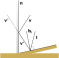
\includegraphics[width=0.4\textwidth]{figures/backvector.pdf}
    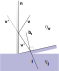
\includegraphics[width=0.4\textwidth]{figures/backvector_refract.pdf}
  \end{center}
  \caption{Geometry of the back-vector for reflection and refraction, illustrated in two dimensions.}
  \label{fig:backvector}
\end{figure}

As illustrated in Figure \ref{fig:backvector}, the reflection $\vecvv$ of the view direction $\vecv$ on the surface can also be interpreted as a reflection of the view direction in a ``virtual'' plane aligned with $\vecv$ and perpendicular to the surface.
Intuitively, this is equivalent to observing the microfacet reflection through a virtual mirror, thus turning glossy forward-reflection into glossy retro-reflection.
While there is no immediate physical foundation to this construction, this interpretation can serve as a motivation why the components of the regular microfacet model still work on changing the domain to the back-vector.
We now detail the mathematical consequences of using the back-vector as microfacet selector.

\paragraph*{Jacobian of Back-Vector.}
First we observe that the Jacobian of the change of variable from the back-vector to the light vector $\vecl$ for specular microfacets~(Equation~(11) and~(14) of \citet{WalterMicrofacet}) has the same form as the half-vector one:
\begin{equation}
\left\lVert \dfrac{\partial \omega_{\vecb_{r}}}{\partial \omega_{\vecl}} \right\rVert = \left\lVert \dfrac{\partial \omega_{\vech_{r}(\vecvv, \vecl)}}{\partial \omega_{\vecl}} \right\rVert = \dfrac{1}{4 \left| \vdot{\vecl}{\vech(\vecvv, \vecl)} \right|} = \dfrac{1}{4 \left| \vdot{\vecl}{\vecb} \right|} \ .
\end{equation}
We also observe that this is true for refractive microfacets~(Equation (17) of \citet{WalterMicrofacet}):
\begin{equation}
\left\lVert \dfrac{\partial \omega_{\vecb_{t}}}{\partial \omega_{\vecl}} \right\rVert = \left\lVert \dfrac{\partial \omega_{\vech_{t}(\vecvv, \vecl)}}{\partial \omega_{\vecl}} \right\rVert = \dfrac{  \eta_o^2 \left| \vecl, \vech_{t}(\vecvv, \vecl)  \right|}{ \left\lVert \vech_{t}(\vecvv, \vecl) \right\rVert^2}
\end{equation}
This is due to the fact that we have to differentiate with respect to the light direction which is not altered by the back vector.

\begin{figure}[tbh]
  \centering
  \includegraphics[width=0.99\linewidth]{figures/brdf_plots.pdf}
  \caption{Comparison of the retro-reflective MRM BRDF (blue) to the regular GGX microfacet BRDF (green) and rough-diffuse EON model (orange), as a function of view direction $\theta_o$ for fixed light directions $\theta_i \in {45^\circ, 80^\circ}$. The dashed lines are the roughness $0.1$ case, and the dashed lines roughness $0.666$. The grey horizontal line at $1/\pi$ is the Lambert BRDF.}
  \label{fig:brdf_plots}
\end{figure}

\paragraph*{Microfacet reflection term.}
There is experimental evidence~\cite{BelcourBackvector} that using a Fresnel term based on the back-vector can provide a good match to actual retro-reflective material measurements for a reflection back-vector based BRDF.
As such, we update the formulation of $\rho(\vecv, \vecm)$~(Equation (11) of \citet{WalterMicrofacet}) to use the reflected view vector instead. From the aforementioned equivalence of the Jacobians, it follows that the reflection microsurface BRDF~(Equation (15) of \citet{WalterMicrofacet}) becomes
\begin{equation}
  f_r^m(\vecv, \vecl, \vecm) = F(\vecvv, \vecm) \dfrac{\delta(\vecb_r, \vecm) }{4 \left| \vdot{\vecvv}{\vecb_r} \right|^2}.
\end{equation}
We used the fact that $\left| \vdot{\vecl}{\vecb} \right| = \left| \vdot{\vecvv}{\vecb} \right|$.
Similarly, for the transmissive microsurfacet BTDF (Equation~(18) of \citet{WalterMicrofacet}) we get
\begin{equation}
  f_t^m(\vecv, \vecl, \vecm) = \left(1-F(\vecvv, \vecm)\right) \dfrac{\delta(\vecb_t, \vecm) \eta_o^2 }{\left( \eta_i \vdot{\vecv^\prime}{\vecb_t} + \eta_o \vdot{\vecl}{\vecb_t} \right)^2}.
\end{equation}

\paragraph*{Shadowing \& Masking.}
We simply apply Smith or v-cavities masking to the mirrored microfacet distribution.
With Smith masking, this is actually identical to a regular microfacet BSDF, as $\vecvv$ and $\vecv$ share the same geometric configuration.
For v-cavities masking, we take $\vecvv$ as view direction and, consequently, $\vecb$ as microfacet normal.
%\todo{\tiny Laurent: I think we could extract the shadowing from Matthias derivation here. The other way to justify the derivation of the full model is to highlight that Smith's shadowing/masking does not depend on the microfacet (appart from the sideness). Hence, whatever the microfacet selector (as long as the sideness matches), the shadowing/masking is the same. Since $\vecv$ and $\vecvv$ share the same slope, we can exchange them in the equation.}

\paragraph*{Final form.}
It follows from all this that the final retro-reflective microfacet model can be written simply as
\begin{equation} \label{eq:retro_microfacet_model}
  %  f_\text{retro}(\vecv, \vecl) = f(\vecvv, \vecl) = \frac{D(\vecb) \, G_{2}(\vecvv,\vecl) \, F(\vecvv, \vecb)}{4 \vdot{\vecvv}{\vecn} \vdot{\vecl}{\vecn}}
  f_\text{retro}(\vecv, \vecl) =
  \begin{cases}
    f_{r, \text{retro}}(\vecv, \vecl) = f_r(\vecvv, \vecl)  & \text{if} \vdot{\vecv}{\vecn}\vdot{\vecl}{\vecn} \geq 0, \\
    f_{t, \text{retro}}(\vecv, \vecl) = f_t(\vecvv, \vecl)  & \text{otherwise}.
  \end{cases}
\end{equation}
In the following section we show in detail that this model is plausible, i.e. that symmetry and energy conservation requirements are fulfilled.
Note that for this we impose one technical assumption on $D$:
we require that the microfacet normal distribution is reflection-symmetric around the normal (which is the case for all isotropic distributions and for anisotropic Phong, Beckmann, and GGX).

Figure~\ref{fig:brdf_plots} plots the BRDF values of the MRM model (green) compared to the rough diffuse (albedo 1) EON model \cite{Portsmouth2025EON} (orange) and GGX (blue). For both MRM and GGX, the Fresnel factor is set to 1.
The $0.1$ roughness case is a very strong, tight peak (note the logarithmic scale on the y-axis), while the $0.666$ roughness case is a much broader peak.
It is evident that MRM BRDF is the same as GGX,with the peak flipped to be back-scattering (at exactly $\theta_o =-\theta_i$, $\phi_o = \phi_i$).
The $\phi_o = 45^\circ$ case demonstrates the situation when the view direction is not aligned in the same azimuthal plane. In this case. both GGX and MRM are dimmer than Lambert or EON, which compensates for the extra energy of the peaks of MRM and GGX (in which almost all of the energy is concentrated, in the reflection or retro-reflection direction respectively for GGX and MRM).


\section{Plausibility of the Back-vector Modification}

\label{sec:plausibility}

In analogy to the notation for $\vecvv$ we generally let $\vecxx := \text{reflect}(\vecx, \vecn)$.
First we observe
\begin{equation}\label{eq:nk}
  \begin{split}
    \vdot{\vecvv}{\vecn} &= \vdot{\vecv}{\vecn} \text{ and}\\
    \vdot{\vecl}{\vecn} &= \vdot{\vecll}{\vecn}.
  \end{split}
\end{equation}
For the reflection back-vector we show $\vechr(\vecvv, \vecl) = \text{reflect}\left(\vechr(\vecll, \vecv), \vecn\right)$, as
\begin{equation}
  \begin{split}
  \vecvv + \vecl &=
  \left(-\vecv + 2 \vdot{\vecv}{\vecn} \vecn \right) + \vecl \\
  &= \left(-\vecv + 2 \vdot{\vecv}{\vecn} \vecn \right) + \left(- \vecll + 2 \vdot{\vecll}{\vecn} \vecn \right)\\
  &= -(\vecll + \vecv) + 2 \vdot{(\vecll + \vecv)}{\vecn} \vecn =
  \text{reflect}(\vecll + \vecv, \vecn) \ .
  \end{split}
\end{equation}
and therefore $\lVert \vecvv + \vecl \rVert = \lVert \vecll + \vecv \rVert$ as well.
Similarly, for refraction we have
\begin{equation}
  \begin{split}
  \etav\vecvv + \etal\vecl &=
  \etav\left(-\vecv + 2 \vdot{\vecv}{\vecn} \vecn \right) + \etal\vecl \\
  &= \etav\left(-\vecv + 2 \vdot{\vecv}{\vecn} \vecn \right) + \etal\left(- \vecll + 2 \vdot{\vecll}{\vecn} \vecn \right)\\
  &= -(\etal\vecll + \etav\vecv) + 2 \vdot{(\etal\vecll + \etav\vecv)}{\vecn} \vecn =
  \text{reflect}(\etal\vecll + \etav\vecv, \vecn) \ .
  \end{split}
\end{equation}
which implies $\lVert \etav\vecvv + \etal\vecl \rVert = \lVert \etal\vecll + \etal\vecv \rVert$ and
results in $\vecht(\vecvv, \vecl) = \text{reflect}\left(\vecht(\vecll, \vecv), \vecn\right)$.
From that we can conclude
\begin{equation}\label{eq:nh}
  \begin{split}
    \vdot{\vecn}{\vech(\vecvv, \vecl)} &=
    \vdot{\vecn}{\vech(\vecll, \vecv)}  \ , \\
    \vdot{\mathbf{t_1}}{\vech(\vecvv, \vecl)} &=
    -\vdot{\mathbf{t_1}}{\vech(\vecll, \vecv)} \ , \\
    \vdot{\mathbf{t_2}}{\vech(\vecvv, \vecl)} &=
    -\vdot{\mathbf{t_2}}{\vech(\vecll, \vecv)}\\
    \end{split}
\end{equation}
for both reflection ($\vech = \vechr$) and refraction ($\vech = \vecht$) cases.
Since we assumed $D$ is reflection-symmetric around the normal, i.e. it takes the form
\begin{equation}
D(\vech) = D\left(\avdot{\vecn}{\vech}, \lvert \vdot{\mathbf{t_1}}{\vech} \rvert, \lvert \vdot{\mathbf{t_2}}{\vech} \rvert\right)
\end{equation}
we can thus infer that using it with a back-vector obeys symmetry.
Further, the reflection symmetry of $D$ along with Equation \eqref{eq:nk} gives
\begin{equation}
  \begin{split}
  G_{1,\text{Smith}}(\vecv, \vech) &=
  \frac{\avdot{\vecv}{\vecn}}{\int_{\lbrace\vech \in \Omega_{\vecv}: \vdot{\vecv}{\vech} \geq 0\rbrace} D(\vech) \vdot{\vecv}{\vech} d\vech} \\
  &= \frac{\avdot{\vecvv}{\vecn}}{\int_{\lbrace\vech \in \Omega_{\vecvv}: \vdot{\vecvv}{\vech} \geq 0\rbrace} D(\vech) \vdot{\vecvv}{\vech} d\vech} =
  G_{1,\text{Smith}}(\vecvv, \vech)
  \end{split}
\end{equation}
for Smith-masking. Next we show
\begin{equation}
  \begin{split}
%  \vdot{\vecx}{\vecy} = -\vdot{\vecxx}{\vecy} + 2 \vdot{\vecxx}{\vecn}\vdot{\vecy}{\vecn}
%  = \vdot{\vecxx}{-\vecyy + 2 \vdot{\vecyy}{\vecn}\vecn} = \vdot{\vecxx}{\vecyy}
    \vdot{\vecxx}{\vecyy} &= \vdot{-\vecx}{\vecyy} + 2 \vdot{\vecx}{\vecn}\vdot{\vecn}{\vecyy}\\
  &= \vdot{-\vecx}{-\vecy} + \vdot{-\vecx}{2 \vdot{\vecy}{\vecn}\vecn} + 2 \vdot{\vecx}{\vecn}\vdot{\vecn}{\vecy}\\
  &= \vdot{\vecx}{\vecy}
\end{split}
\end{equation}
and therefore
\begin{equation}\label{eq:khr}
  \vdot{\vecx}{\vech(\vecx, \vecy)} =
  \frac{1 + \vdot{\vecy}{\vecx}}{\lVert \vecx + \vecy \rVert} =
  \frac{\vdot{\vecyy}{\vecyy} + \vdot{\vecyy}{\vecxx}}{\lVert \vecyy + \vecxx \rVert} =
  \vdot{\vecyy}{\vech(\vecyy,\vecxx)}
\end{equation}
as well as
\begin{equation}\label{eq:kht}
  \vdot{\vecx}{\vecht(\vecx, \vecy)} =
  \frac{-\etax  -\etay \vdot{\vecx}{\vecy}}{\lVert -\etax\vecx  -\etay\vecy \rVert} =
  \frac{-\etax \vdot{\vecyy}{\vecyy} - \etay\vdot{\vecxx}{\vecyy}}{\lVert -\etax\vecxx  -\etay\vecyy \rVert} =
  \vdot{\vecyy}{\vech(\vecyy,\vecxx)}.
\end{equation}
As the Fresnel term takes the form $F(\vecx, \vecy) = F\left(\vdot{\vecx}{\vecy}\right)$, we can conclude
  \begin{equation}
    F\left(\vecvv, \vech(\vecvv, \vecl)\right) = F\left(\vdot{\vecvv}{\vech(\vecvv, \vecl)}\right) =
    F\left(\vdot{\vecll}{\vech(\vecll,\vecv)}\right) = F\left(\vecll, \vech(\vecll,\vecv)\right).
\end{equation}
Getting back to the geometry term, we first note that we can rewrite $G_1(\vecv, \vech)$ as $G_1(\vecv, \vech(\vecv, \vecl))$. For ease, we change the notation to $G_1(\vecv, \vecl)$ instead of $G_1(\vecv, \vech)$, and $G_1(\vecl, \vecv)$ instead of $G_1(\vecl, \vech)$. It follows that using Equations \eqref{eq:khr} and \eqref{eq:kht} along with Equations \eqref{eq:nh} and \eqref{eq:nk} und using $\vech(\vecx,\vecy) = \vech(\vecy,\vecx)$ we get
\begin{equation}
  \begin{split}
  G_1(\vecvv, \vecl) &=
  G_{1, \text{vc}}\left( \vdot{\vecvv}{\vecn}, \vdot{\vecn}{\vech(\vecvv, \vecl)}, \vdot{\vecvv}{\vech(\vecvv, \vecl)} \right)\\
  &=  G_{1, \text{vc}}\left( \vdot{\vecv}{\vecn}, \vdot{\vecn}{\vech(\vecll, \vecv)}, \vdot{\vecll}{\vech(\vecll, \vecv)} \right) \\
  &=  G_{1, \text{vc}}\left( \vdot{\vecv}{\vecn}, \vdot{\vecn}{\vech(\vecv, \vecll)}, \vdot{\vecll}{\vech(\vecv, \vecll)} \right) \\
  &= G_1(\vecv, \vecll)
  \end{split}
\end{equation}
and similarly $G_1(\vecl, \vecvv) = G_1(\vecll, \vecv)$ for the V-cavity masking function.
In summary, we can conclude the reciprocity symmetry of the BRDF
\begin{equation}
  \begin{split}
  f_{r,\text{retro}}(\vecv, \vecl) =
  f_r(\vecvv, \vecl) &=
  \frac{D(\vech(\vecvv, \vecl)) G_{2}(G_1(\vecvv, \vecl), G_1(\vecl, \vecvv)) F(\vecvv, \vecl)}{4 \vdot{\vecvv}{\vecn} \vdot{\vecl}{\vecn} }\\
  &=
  \frac{D(\vech(\vecll, \vecv)) G_{2}(G_1(\vecv, \vecll), G_1(\vecll, \vecv)) F(\vecll, \vecv)}{4 \vdot{\vecv}{\vecn} \vdot{\vecll}{\vecn} }\\
  &=
  f_r(\vecll, \vecv) =
  f_{r,\text{retro}}(\vecl, \vecv).
  \end{split}
\end{equation}
Analogously, we obtain the reciprocity symmetry requirement of the BTDF
\begin{equation}
  \begin{split}
    &f_{t,\text{retro}}(\vecv, \vecl)
    =  f_t(\vecvv, \vecl)\\
    &= \frac{\avdot{\vecvv}{\vecht(\vecvv, \vecl)}\avdot{\vecl}{\vecht(\vecvv, \vecl)}\etav^2 D(\vecht(\vecvv, \vecl)) \, G_{2}(\vecvv,\vecl) \, \left(1 - F(\vecvv, \vecht(\vecvv, \vecl)) \right)}
    {\avdot{\vecvv}{\vecn} \avdot{\vecl}{\vecn} \left(\etav \vdot{\vecvv}{\vecht(\vecvv, \vecl)} + \etal \vdot{\vecl}{\vecht(\vecvv, \vecl)}\right)^2} \\
    &= \frac{\avdot{\vecv}{\vecht(\vecv, \vecll)}\avdot{\vecll}{\vecht(\vecv, \vecll)}\etav^2 D(\vecht(\vecll, \vecv)) \, G_{2}(\vecll,\vecv) \, \left(1 - F(\vecll, \vecht(\vecll, \vecv)) \right)}
    {\avdot{\vecv}{\vecn} \avdot{\vecll}{\vecn} \left(\etav \vdot{\vecv}{\vecht(\vecv, \vecll)} + \etal \vdot{\vecll}{\vecht(\vecv, \vecll)}\right)^2} \\
    &=
    \frac{\etav^2}{\etal^2}f_t(\vecll, \vecv) =
    \frac{\etav^2}{\etal^2}f_{t,\text{retro}}(\vecl, \vecv).
  \end{split}
\end{equation}
For the directional albedos we simply have
\begin{equation}
  \begin{split}
  \rho_{r, \text{retro}}(\vecv) =
  \int_{\Omega_{\vecv}} f_{r, \text{retro}}(\vecv, \vecl) \vdot{\vecl}{\vecn} d\vecl =
  \int_{\Omega_{\vecvv}} f_r(\vecvv, \vecl) \vdot{\vecl}{\vecn} d\vecl = \rho_r(\vecvv),\\
  \rho_{t, \text{retro}}(\vecv) =
  \int_{\Omega_{-\vecv}} f_{t, \text{retro}}(\vecv, \vecl) \avdot{\vecl}{\vecn} d\vecl =
  \int_{\Omega_{-\vecvv}} f_t(\vecvv, \vecl) \avdot{\vecl}{\vecn} d\vecl = \rho_t(\vecvv),
  \end{split}
\end{equation}
i.e. we get the albedo of the regular microfacet BSDF for the reflected direction.
As the original microfacet BSDF fulfills energy conversion, the retro-reflective modification does, too.
%% Which, using equation \eqref{eq:visible} and $\frac{d\vech(\vecvv, \vecl)}{d\vecl} = \frac{1}{4 \vdot{\vecl}{\vech(\vecvv, \vecl)}}= \frac{1}{4 \vdot{\vecvv}{\vech(\vecvv, \vecl)}}$ \cite{WalterMicrofacet}, can be shown to fulfill energy conservation
%% \begin{equation}
%%   \begin{split}
%%   \rho(\vecvv) &=
%%   \int_\Omega \frac{D(\vech(\vecvv, \vecl)) G_{2}(\vecvv,\vecl)}{4 \vdot{\vecvv}{\vecn} \vdot{\vecl}{\vecn}}\vdot{\vecl}{\vecn} d\vecl\\
%%   &\leq
%%   \int_{\lbrace\vech \in \Omega: \vdot{\vecvv}{\vech} \geq 0\rbrace} \frac{D(\vech) G_1(\vecvv,\text{reflect}(\vecvv, \vech))}{\vdot{\vecvv}{\vecn}}\vdot{\vecvv}{\vech} d\vech
%%   = 1.
%%   \end{split}
%% \end{equation}
We further note that under our requirement of a reflection-symmetric microfacet normal distribution, the geometric
configurations for $\vecv$ and $\vecvv$ are identical.
Hence we can conclude $\rho_r(\vecv) = \rho_r(\vecvv)$ and $\rho_t(\vecv) = \rho_t(\vecvv)$, which in turn implies that the albedos of forward and retro-reflection are the same, i.e. $\rho_{r, \text{retro}}(\vecv) = \rho_r(\vecv)$ and $\rho_{t, \text{retro}}(\vecv) = \rho_t(\vecv)$.


\section{Implementation Notes}
\label{sec:implementation}

Given an implementation of a regular microfacet BSDF, extending it to retro-reflection is extremely straightforward (see the pseudo-code provided in Listing~\ref{lst:implementation}):

\begin{itemize}
\item
  Evaluation merely needs to replace $\vecv$ with $\vecvv$ upfront.
\item
  Similarly, importance sampling of $\vecl$ given $\vecv$ can be realized by replacing $\vecv$ with $\vecvv$ upfront and then importance sampling the regular microfacet BSDF.
  This may include low variance sampling using the domain of visible microfacets \cite{HeitzIS}.
\item
  As the albedos of standard BSDF and retro-reflective BSDF are identical, compensating for energy loss in the sense of \cite{KelemenBRDF} can be realized using the same data tables.
\end{itemize}

\noindent
\begin{lstlisting}[
    style=snippet,
    language=GLSL,
    caption=Pseudo code to implement the retro-reflective microfacet model using an existing regular microfacet BSDF implementation,
    label=lst:implementation,
    nolol=true,
    frame=trBL
    ]
Sample_result sample_bsdf_retro(vec3 V, vec3 L, vec3 N, Bsdf_params params)
{
    vec3 Vp = -V + 2.0 * dot(V, N) * N;
    return sample_bsdf(Vp, L, N, params);
}
Eval_result eval_bsdf_retro(vec3 V, vec3 L, vec3 N, Bsdf_params params)
{
    vec3 Vp = -V + 2.0 * dot(V, N) * N;
    return eval_bsdf(Vp, L, N, params);
}
\end{lstlisting}




\section{Results and Discussion}

\label{sec:results}

\paragraph*{Incorporation in a standard microfacet model}

Figure~\ref{fig:conductor_renders} shows renders of a shaderball with either a classic GGX or retro-reflective MRM material applied, here assuming \emph{conducting} (i.e. metallic) microfacets.

\paragraph*{Combination of BRDF and BTDF}

The albedo is identical for forward- and retro-reflective BRDF as well as BTDF, which allows to arbitrarily combine forward- and retro-reflective variants into a BSDF.
When constructing an artist-controllable retro-reflective dielectric BSDF, we observed that using $f_t$ instead of $f_{t, \text{retro}}$ yields more intuitive results, in particular for an index of refraction close to 1.

Figure~\ref{fig:dielectric_renders} demonstrates this in renders of a dielectric shaderball, where the IOR of the dielectric material is either $1.0$ (top row) or $1.5$ (bottom row).
Left to right we show three combinations of BRDF and BTDF: the classic microfacet BSDF $f_r$ and BTDF $f_t$ (left), the retro-reflective BRDF $f_{r,\text{retro}}$ plus retro-reflective BTDF $f_{t,\text{retro}}$ (middle), and retro-reflective BRDF $f_{r,\text{retro}}$ combined with the classic (non-retroreflective) BTDF $f_t$ (right).

\begin{figure}[!ht]
    \centering
    \includegraphics[width=0.3\linewidth]{figures/conductor/cropped/classic_angle_0_cropped.png}
    \includegraphics[width=0.3\linewidth]{figures/conductor/cropped/classic_angle_45_cropped.png}
    \includegraphics[width=0.3\linewidth]{figures/conductor/cropped/classic_angle_90_cropped.png} \\
    \vspace{0.06cm}
    \includegraphics[width=0.3\linewidth]{figures/conductor/cropped/retro_angle_0_cropped.png}
    \includegraphics[width=0.3\linewidth]{figures/conductor/cropped/retro_angle_45_cropped.png}
    \includegraphics[width=0.3\linewidth]{figures/conductor/cropped/retro_angle_90_cropped.png}
  \captionsetup{font=small}
  \caption{Renders of a metallic shaderball with either a classic GGX (top row) or retro-reflective MRM material (bottom row) applied, for various camera angles and a fixed light direction. The relative angle between the view and light direction is $0^\circ$ (left), $45^\circ$ (middle), and $90^\circ$ (right). \vspace{-0.5cm}}
  \label{fig:conductor_renders}
\end{figure}

\begin{figure}[!hb]
  \centering
  \begin{tikzpicture}[font=\footnotesize]
    \node[inner sep=1pt] (Class1) {\includegraphics[width=0.3\linewidth,frame]{figures/dielectric/cropped/classic_ior_1_cropped_label.png }};
    \node[inner sep=1pt,right = 0cm of Class1] (MRM1) {\includegraphics[width=0.3\linewidth,frame]{figures/dielectric/cropped/retroRT_ior_1_cropped_label.png }};
    \node[inner sep=1pt,right = 0cm of MRM1] (Mixed1) {\includegraphics[width=0.3\linewidth,frame]{figures/dielectric/cropped/retroR_ior_1_cropped_label.png }};

    \node[inner sep=1pt,below = 0cm of Class1] (Class15) {\includegraphics[width=0.3\linewidth,frame]{figures/dielectric/cropped/classic_ior_1.5_cropped_label.png }};
    \node[inner sep=1pt,right = 0cm of Class15] (MRM15) {\includegraphics[width=0.3\linewidth,frame]{figures/dielectric/cropped/retroRT_ior_1.5_cropped_label.png }};
    \node[inner sep=1pt,right = 0cm of MRM15] (Mixed15) {\includegraphics[width=0.3\linewidth,frame]{figures/dielectric/cropped/retroR_ior_1.5_cropped_label.png }};

    \node[inner sep=1pt,above = 2pt of Class1] { \textbf{Classical Microfacet} };
    \node[inner sep=1pt,above = 2pt of MRM1] { \textbf{Full retro-reflective MRM} };
    \node[inner sep=1pt,above = 11.5pt of Mixed1] { \textbf{Mixed MRM (BRDF)} };
    \node[inner sep=1pt,above = 0.5pt of Mixed1] { \textbf{and Classical (BTDF)} };

    \node[inner sep=1pt,left = 1pt of Class1, anchor=south,rotate=90] { $\mathbf{\boldsymbol{\eta} = 1}$ };
    \node[inner sep=1pt,left = 1pt of Class15, anchor=south,rotate=90] { $\mathbf{\boldsymbol{\eta} = 1.5}$ };
  \end{tikzpicture}

    % \includegraphics[width=0.3\linewidth]{figures/dielectric/cropped/classic_ior_1_cropped_label.png }
    % \includegraphics[width=0.3\linewidth]{figures/dielectric/cropped/retroRT_ior_1_cropped_label.png }
    % \includegraphics[width=0.3\linewidth]{figures/dielectric/cropped/retroR_ior_1_cropped_label.png } \\
    % \vspace{0.06cm}
    % \includegraphics[width=0.3\linewidth]{figures/dielectric/cropped/classic_ior_1.5_cropped_label.png }
    % \includegraphics[width=0.3\linewidth]{figures/dielectric/cropped/retroRT_ior_1.5_cropped_label.png}
    % \includegraphics[width=0.3\linewidth]{figures/dielectric/cropped/retroR_ior_1.5_cropped_label.png }
  \caption{Renders of a glass shaderball illuminated from the side. The index of refraction is $1.0$ (top) or $1.5$ (bottom). From left to right: classic microfacet BSDF (left), retro-reflective BSDF (middle), and combined retro-reflective BRDF and classic BTDF (right).  }
  \label{fig:dielectric_renders}
\end{figure}



\section{Conclusion}

We have presented a retro-reflective microfacet model (MRM) based on a simple modification of the classic microfacet BSDF.
The model is straightforward to implement in existing renderers supporting microfacet BSDFs, as it only requires reflecting the view direction about the surface normal before evaluating the standard microfacet model.
We have shown that the model fulfills symmetry and energy conservation requirements, making it a plausible microfacet model.
The retro-reflective microfacet model can be used to represent materials with strong retro-reflective properties, such as certain fabrics or retro-reflective coatings.


\paragraph{Further work.}
For future work it would be interesting to further validate the MRM retro-reflective microfacet model against measured retro-reflective materials.


\bibliographystyle{jcgt}
\bibliography{citations}

\section*{Author Contact Information}

\hspace{-2mm}\begin{tabular}{p{0.48\textwidth}p{0.48\textwidth}}
Matthias Raab \newline
\href{mailto:mraab@nvidia.com}{mraab@nvidia.com} \newline
&
Laurent Belcour \newline
\href{mailto:laurent.belcour@gmail.com}{laurent.belcour@gmail.com} \\
Frankie Liu \newline
\href{mailto:frankie.liu@gmail.com}{frankie.liu@gmail.com} \newline
&
Jamie Portsmouth \newline
\href{mailto:jamports@mac.com}{jamports@mac.com} \newline
\end{tabular}


\end{document}


